\chapter{Benchmark cases and evaluation methodology}
\label{chap:evaluation-methodology}
Assessing wall-function performance requires consistent reference data, sufficiently resolved RANS baselines and explicit accuracy targets. This chapter introduces the selected zero-pressure-gradient (ZPG) flat-plate (FP) DNS benchmarks and their limitations, specifies the matching procedure and wall-resolved mesh requirements, and defines the criteria used to judge the results. These choices underpin the successive comparisons of turbulence modelling, wall-function closure and mesh sensitivity in Chapter~\ref{chap:comparative-evaluation}.

\section{Selected zero-pressure-gradient flat-plate DNS reference cases}
\label{sec:evaluation:benchmark-cases}

In this chapter the selected fully turbulent zero-pressure-gradient (ZPG) flat-plate (FP) cases used as references for the assessment of the aerothermal heating are being introduced as well as argued why they were chosen, or certain cases neglected. Furthermore in the respective subsections to each of the four primary sources of the DNS references, specific considerations that must be taken into account are highlighted.
\par\medskip

The four primary DNS references are from part 2 \cite{duan2010direct_part2} and part 4 \cite{duan2011direct_Part4} of Martin, Duan et al's four part series (further noted as "Martin-Duan Part 2" and "Martin-Duan Part 4" respectively) , Zhang et al \cite{zhang2018direct} and Huang et al \cite{huang2020simulation}. The selected benchmarks comprise 12 distinct ZPG flat-plate cases, summarized in Table \ref{tab:evaluation:selected-cases}.
\begin{table}[H]
    \centering
    \caption{Selected ZPG flat-plate DNS benchmark cases.}
    \label{tab:evaluation:selected-cases}
    \begin{tabular}{@{}lp{0.62\linewidth}@{}}
        \toprule
        DNS reference & Selected cases \\
        \midrule
        Martin-Duan Part 2 &
        M5T1, M5T2, M5T3, M5T4, M5T5 (adiabatic) \\
        \addlinespace
        Martin-Duan Part 4 &
        LowH\_M3 \\
        \addlinespace
        Zhang &
        M2p5 (adiabatic), M6Tw025, M6Tw076*,
        M8Tw048, M14Tw018 \\
        \addlinespace
        Huang &
        M11Tw020 (stations BL1, BL2, and BL3) \\
        \bottomrule
    \end{tabular}
\end{table}

Case names are retained from the respective publications. The number after \(M\) indicates the nominal freestream Mach number, \(T\) distinguishes the wall-temperature variants in Martin--Duan Part~2. Their thermal conditions are taken from the reported data rather than inferred from the case names. For Zhang and Huang, \(Tw\) denotes the wall-to-recovery temperature ratio \(T_w/T_r\), with recovery factor \(r=0.89\)~\cite[Nomenclature]{zhang2018direct}. Huang's M11Tw020 case is sampled at three downstream stations, BL1--BL3. The asterisk marks the M6Tw076 temperature note below.
\par\medskip

These cases were selected as suitable references because they span a wide range of super- to hypersonic cold-wall regime as well as varying degrees of compressibility as indicated in Figure~\ref{fig:evaluation:dns-bq-mtau} range on the heat-transfer coefficient \(-B_q\) and friction Mach number \(M_\tau\) respectively. \(M_\tau\) is discussed by Smits and Dussauge~\cite{smits2006turbulent} and used here as an indicator for intrinsic compressibility effects, following Hasan et al.~\cite{hasan2025intrinsic}. With cold-wall and compressibility effects seemingly being the dominant factors differentiating hypersonic cold-wall boundary layers from incompressible ones, it was chosen to plot Figure~\ref{fig:evaluation:dns-bq-mtau} using \(-B_q\) and \(M_\tau\). The selected DNS cases don't span the whole  \(-B_q\)-\(M_\tau\) domain and mainly lie clustered on a line. This could partly be attributed to the fact that the friction velocity \(u_\tau\) is scaling both axes, or it may represent a genuine gap in DNS references which may yield interesting insights. To fully judge and address the real-world extend findings based on these DNS references can be applied, further variables such as a Reynolds number might add important value too, so as not to extrapolate findings of this work into non-applicable domains.
\par\medskip

For the cases by Zhang et al it should be positively highlighted that the data has been additionally published digitally at \url{https://tmbwg.github.io/turbmodels/Other_DNS_Data/supersonic_hypersonic_flatplate.html} [accessed 14 September 2026], although the first reported off-wall data point is already at a y\(^+ = 0.5\).

\begin{figure}[H]
    \centering
    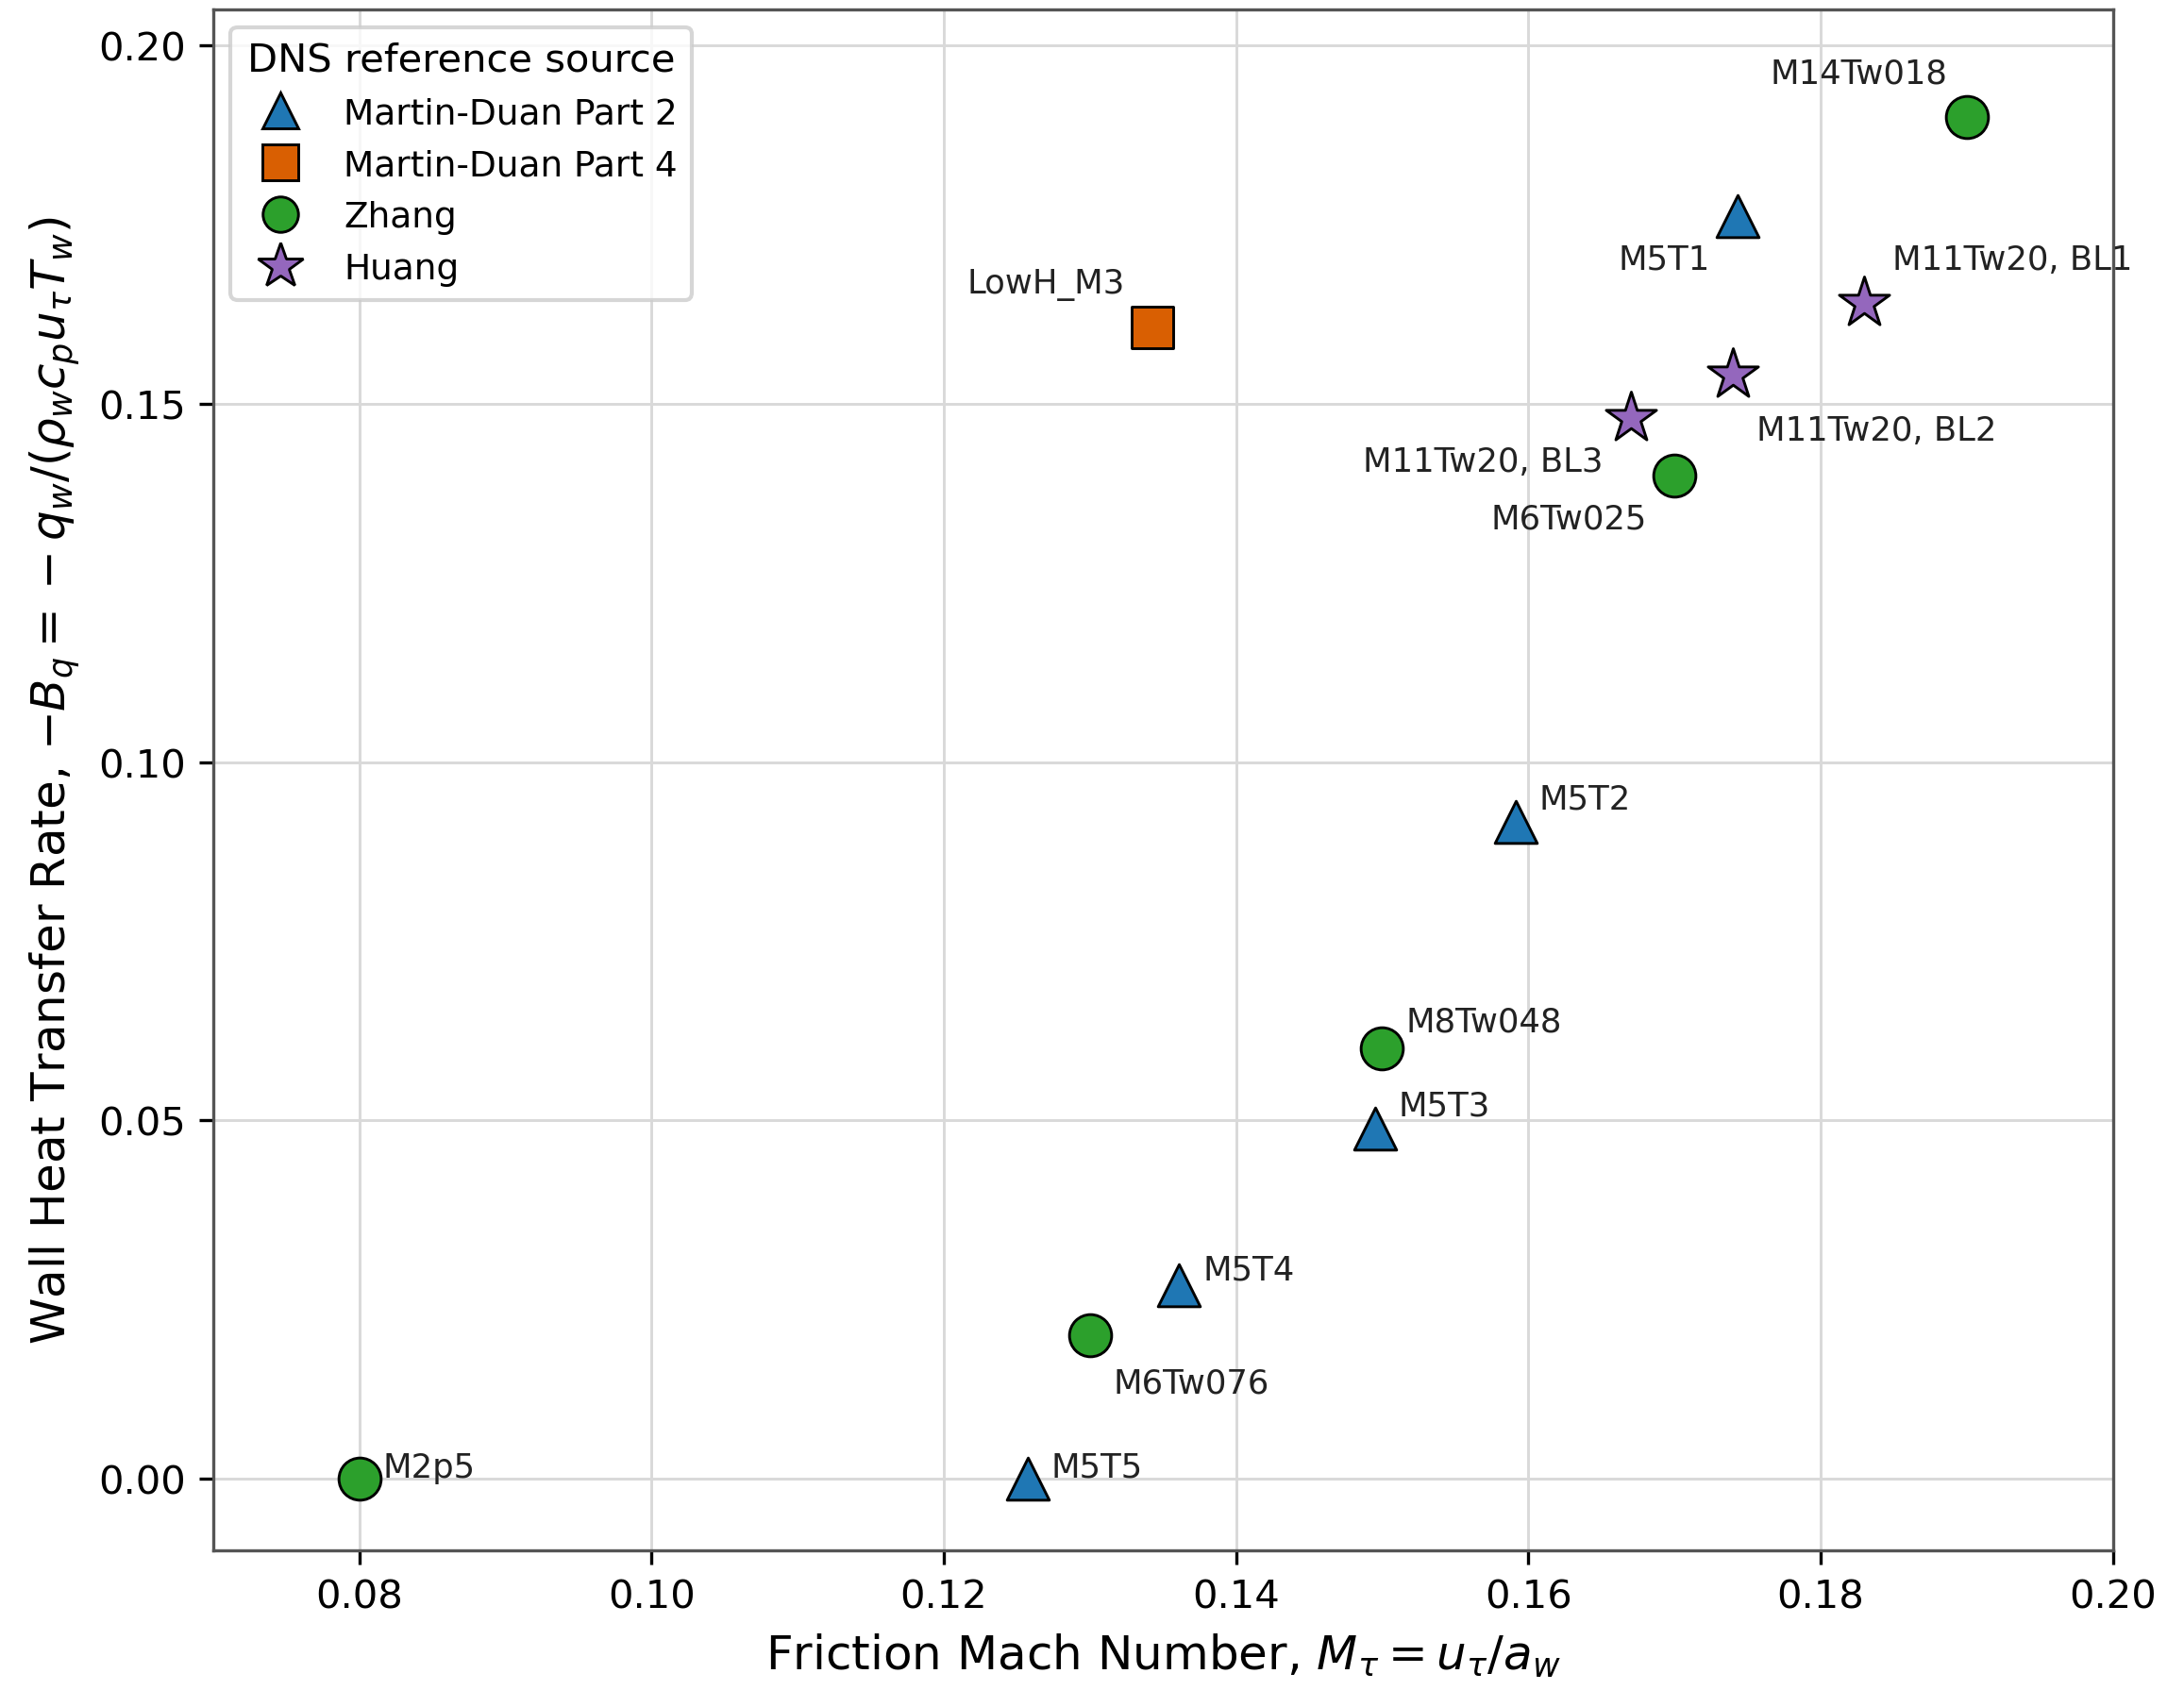
\includegraphics[width=\linewidth]{06_Eval_Methodology/06_Figures/DNS_minus_Bq_vs_M_tau (2).png}
    \caption{Selected DNS benchmark cases in terms of the dimensionless wall heat-transfer rate \(-B_q\) and friction Mach number \(M_\tau\).}
    \label{fig:evaluation:dns-bq-mtau}
\end{figure}

To put the cold-wall strengths of the twelve investigated ZPG flat-plates into perspective of real world flight conditions, the fraction \(\frac{T_w}{T_{r}}\) of the DLR's flight experiment STORT is looked at, where \(T_r\) is the adiabatic recovery temperature. The heat-transfer rate \(-B_q\) is arguably a more comparable assessment of the cold-wall effects, but with flight experiments the skin-friction is rarely if ever available. For the calculation of the \(\frac{T_w}{T_r}\) during the STORT flight, the published thermo couple readings of the surface temperature on the nose cone at 40, 152.1 and 150.5 mm from the nose tip \cite[Figure 10]{reimer2025stort} and the flight Mach numbers \cite[Figure 9 (b)]{reimer2025stort} are used. For simplification, and as this shall only serve as a rough estimation and insight to real world flight, perfect gas with \(\gamma = 1.4\) and a recovery factor of \(r = 0.89\) is assumed. Furthermore the calculations are simplified in assuming the freestream conditions as the boundary layer edge quantities, which is fine for ZPG flat-plates, but with the temperature probes sitting on the nosecone and somewhat close to the nose's bow shock it is arguably a rough engineering approximation, but measurements or high fidelity simulation results of the actual temperature boundary layer are not available. Thus figure should be understood as an indicative plot and not as an exact categorization of the cold-wall strength the STORT flight experienced. Never the less Figure \ref{fig:evaluation:stort-Twall-Tad} shows that \(\frac{T_w}{T_r}\) ratios of e.g. 0.25, like herein investigated in the M6Tw025 ZPG flat-plate, are not extraordinarily cold-walls, and well within what a hypersonic vehicle can experience. But when looking at validation of RANS models, adiabatic or even slightly warm walls (i.e. negative heat-flux, from the wall to the fluid) are to be looked at, but then again it all is very case-by-case dependant on the material, or trajectory.

\begin{figure}[H]
    \centering
    % Notation-only regeneration (2026-10-19): T_ad -> T_r in display labels.
    % Source: /home/mgnadlinger/ZPG_FP_overview/STORT/recovery_temperature/plot_stort_recovery.py
    % Data: /home/mgnadlinger/ZPG_FP_overview/STORT/STORT_experiment_data.xlsx
    % Wrapper/audit: tmp/notation_figures_20261019/regenerate_stort.py and stort_audit.json.
    % Prior notation-only pass retained the original manuscript crop and image dimensions.
    % Caption-sized font regeneration (2026-10-19): 10 pt at 170 mm manuscript width.
    % Reproducible script: 06_Figures/plot_stort_caption_fonts.py; archived original
    % script/workbook and numerical/layout audit: 06_Figures/stort_sources/.
    % All plotted samples, axes limits and the calculation CSV are unchanged.
    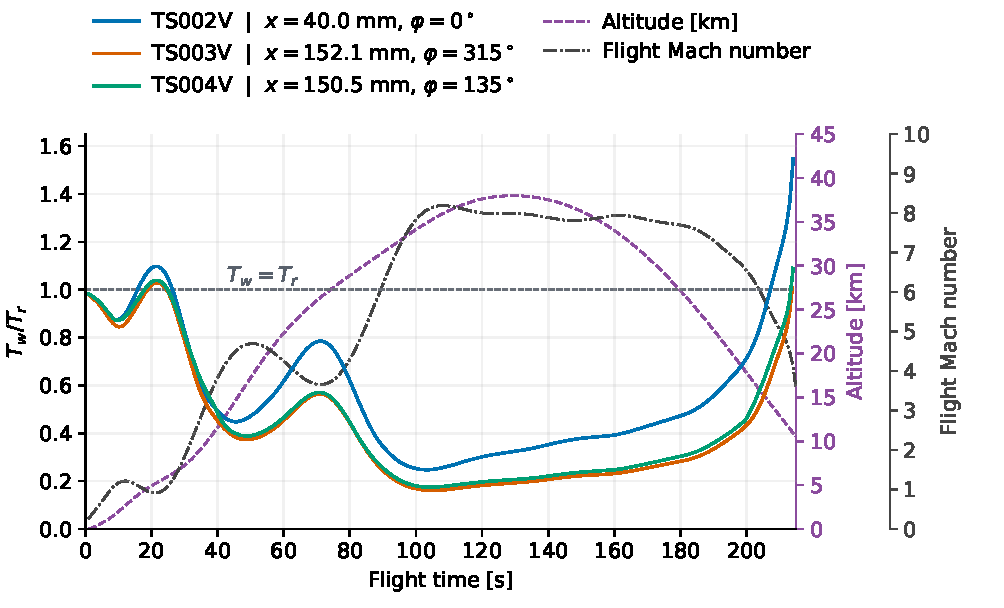
\includegraphics[width=\linewidth]{06_Eval_Methodology/06_Figures/STORT_Twall_Tad.pdf}
    \caption{Indicative \(T_w/T_r\) ratio experienced by the DLR's STORT hypersonic flight experiment \cite{gulhan2022objectives}. TS002V, TS003V and TS004V are the surface thermal couples as reported in \cite{reimer2025stort}, with their location on the nose cone, as measured in millimetres from the nose tip.}
    \label{fig:evaluation:stort-Twall-Tad}
\end{figure}

\subsection{Inflow and wall conditions}

In this section the inflow and wall conditions of the reference DNS cases are extracted from the respective sources and discussed. For this work it was elected to assign the reported freestream conditions, as reported in the tables below, at the inlet in a uniform manner. In \ref{subsec:comparative:zpg:results-assessment} a publication by Vaughen argued for using back calculated pre-shock conditions instead - a sensitivity analysis was performed and revealed limited affect and no clear claim of which approach, DNS freestream or back calculated pre-shock values are a more correct replication of the DNS cases. 

\paragraph*{Martin-Duan}

Martin-Duan Part 2 and Martin-Duan Part 4 are both created using an initial RANS simulation with added transformed DNS fluctuations followed by a recycling scheme to develop the boundary layer along the flat-plate temporally with streamwise periodic boundary conditions \cite{martin2007direct_Part1}. The inflow conditions selected are taken from the reported freestream conditions for the Mach 5 case in Table 1 of \cite{martin2007direct_Part1}, which are reiterated or derived from it here in Table \ref{tab:evaluation:martin-duan-inflow-wall}, similarly for the LowH\_M3 case the freestream conditions are defined in \cite[Table 1]{duan2011direct_Part4}. The only difference in the M5T1 to M5T5 cases are the isothermal wall temperature.
\par\medskip

Martin-Duan Part 4 contains additional reacting references cases, which are beyond the scope of this work, and additionally a calorically and thermally perfect case, named LowH\_M10. This case is intentionally omitted because of it represents an incredibly far downstream station as a result of multiple recycling which leads to an over 1.3 metre thick boundary layer at the matching station \cite[Table 2]{duan2011direct_Part4}. This is also highlighted by the authors themselves, and noted that “the flow conditions themselves might not be realistic” \cite{duan2011direct_Part4}.

\begin{table}[H]
    \centering
    \caption{Freestream inflow and wall conditions for the Martin-Duan cases.}
    \label{tab:evaluation:martin-duan-inflow-wall}
    \begin{tabular}{l S[table-format=1.2] S[table-format=1.4] S[table-format=3.2] S[table-format=4.2]}
        \toprule
        Case & {\(M_\infty\)} & {\(\rho_\infty\;[\mathrm{kg}/\mathrm{m}^3]\)} & {\(T_\infty\;[\mathrm{K}]\)} & {\(T_w\;[\mathrm{K}]\)} \\
        \midrule
        M5T1 & 5.00 & 0.0889 & 216.65 & 228.1 \\
        M5T2 & 5.00 & 0.0889 & 216.65 & 433.30 \\
        M5T3 & 5.00 & 0.0889 & 216.65 & 649.95 \\
        M5T4 & 5.00 & 0.0889 & 216.65 & 866.60 \\
        M5T5 & 5.00 & 0.0889 & 216.65 & 1191.6 \\
        LowH\_M3 & 3.5 & 0.0184 & 226.5 & 125 \\
        \bottomrule
    \end{tabular}
\end{table}

For M5T1, the prescribed wall temperature \(T_w=228.1\,\mathrm{K}\) follows Part~2 Table~1, which gives \(T_w/T_\delta=1.00\) and \(T_\delta=228.1\,\mathrm{K}\)~\cite{duan2010direct_part2}. The separate Reynolds-number inconsistency is examined in Appendix~\ref{app:duan-part2-consistency}.

\paragraph*{Zhang}

Zhang et al.’s DNS database comprises spatially developing flat-plate turbulent boundary layers with turbulent inflow supplied by a modified recycling/rescaling method. An extended downstream development region allows artificial effects of inflow generation to decay before statistics are evaluated \cite{zhang2018direct}. The cases were selected in a way to represent various experimental hypersonic wind tunnel experimental conditions. The freestream inflow quantities are taken from \cite[Tbale 1]{zhang2018direct} and reiterated here in Table \ref{tab:evaluation:zhang-inflow-wall}.

\begin{table}[H]
    \centering
    \caption{Freestream inflow and wall conditions for the Zhang cases.}
    \label{tab:evaluation:zhang-inflow-wall}
    \begin{tabular}{l S[table-format=2.2] S[table-format=1.3] S[table-format=3.1] S[table-format=3.1,table-space-text-post={*},table-align-text-after=false]}
        \toprule
        Case & {\(M_\infty\)} & {\(\rho_\infty\;[\mathrm{kg}/\mathrm{m}^3]\)} & {\(T_\infty\;[\mathrm{K}]\)} & {\(T_w\;[\mathrm{K}]\)} \\
        \midrule
        M2P5 & 2.50 & 0.100 & 270.0 & {(adiabatic)} \\
        M6Tw025 & 5.84 & 0.044 & 55.2 & 97.5 \\
        M6Tw076 & 5.86 & 0.043 & 55.0 & 300.0{*} \\
        M8Tw048 & 7.87 & 0.026 & 51.8 & 298.0 \\
        M14Tw018 & 13.64 & 0.017 & 47.4 & 300.0 \\
        \bottomrule
    \end{tabular}
\end{table}

The asterisk ``*'' on the M6Tw076 case's \(T_w\) comes from an inconsistency between the paper's Table 1 reported \(T_w = 300 K\) and the digitally published boundary profile data which at the wall face (\(z = 0\)), reports a \(T/T_\infty = 5.38\), which, with the paper's Table 1 reported \(T_\infty = 55.0 \mathrm{K}\), results in a \(T_w = 295.9 \mathrm{K}\). This \(4 \mathrm{K}\) is a minor inconsistency, but in some Temperature related plots is a visible. Furthermore, with the M6Tw076 being almost adiabatic with a reported \(-B_q = 0.02\) \cite[Table 2]{zhang2018direct}, this wall temperature deviation can carry a higher than expected uncertainty for the wall heat-flux.

\paragraph*{Huang}

Huang et al use a precursor RANS simulation similar to Duan and Martin, with turbulent inflow generated by recycling/rescaling and subsequently spatially developing boundary layer through three overlapping DNS boxes. The freestream and isothermal wall-temperature conditions are taken from the reported Table 1 in \cite{huang2020simulation}.

\begin{table}[H]
    \centering
    \caption{Freestream inflow and wall conditions for the Huang case.}
    \label{tab:evaluation:huang-inflow-wall}
    \begin{tabular}{l S[table-format=2.1] S[table-format=1.3] S[table-format=2.1] S[table-format=3.0]}
        \toprule
        Case & {\(M_\infty\)} & {\(\rho_\infty\;[\mathrm{kg}/\mathrm{m}^3]\)} & {\(T_\infty\;[\mathrm{K}]\)} & {\(T_w\;[\mathrm{K}]\)} \\
        \midrule
        M11Tw020 & 10.9 & 0.103 & 66.5 & 300 \\
        \bottomrule
    \end{tabular}
\end{table}

\subsection{Thermal and transport models}

All of the investigated DNS references herein represent thermally and calorically perfect gases. With the exception of the M8Tw048 case, which represent pure Nitrogen, all of the DNS references represent air.

\begin{table}[H]
    \centering
    \caption{Thermal models defined in or reasonably inferrable from the DNS references.}
    \label{tab:evaluation:thermal-models}
    \begin{tabular}{l S[table-format=4.2,table-space-text-post={*},table-align-text-after=false] S[table-format=1.1,table-space-text-post={*},table-align-text-after=false] S[table-format=3.2,table-space-text-post={*},table-align-text-after=false] S[table-format=1.2]}
        \toprule
        Case & {\(c_{p,\infty}\;[\mathrm{J}/\mathrm{kg\,K}]\)} & {\(\gamma_\infty\)} & {\(R\;[\mathrm{J}/\mathrm{kg\,K}]\)} & {\(Pr\)} \\
        \midrule
        Martin-Duan Part 2/4 & 1004.5 & 1.4 & 287 & {(not defined)} \\
        Zhang & 1004.5 & 1.4 & 287 & 0.71 \\
        Zhang - M8Tw048 & 1039.68{*} & 1.4{*} & 297.05{*} & 0.71 \\
        Huang & 1004.5 & 1.4 & 287 & 0.71 \\
        \bottomrule
    \end{tabular}
\end{table}

The Martin-Duan cases leave the most ambiguity, as throughout their four part series they only ever state "the working fluid is air" \cite[p. 422]{duan2010direct_part2}. For the molecular Prandtl number, Martin and Duan give no explicit value or a law for the conductivity law to infer it. It was chosen to go with a \(Pr = 0.71\) as the other references also do so and it is a common value to use for perfect air.
\par\medskip

The asterisk ``*'' on the M8Tw048 case is because it suffers similar ambiguity, where the \(\gamma\), \(R\) or \(c_p\) are not defined, rather the \(\gamma \) must be derived through the given recovery temperature ratio. Subsequently, through \(\frac{M}{U_\infty} = \sqrt{\gamma R T}\) and \(c_p = \frac{\gamma R}{\gamma - 1}\), the thermal gas model can be fully inferred, with the specific gas constant for diatomic Nitrogen given as \(R = 296.803 \mathrm{J}/\mathrm{kg\,K}\) by NIST\footnote{[accessed 14 September 2026] \url{https://webbook.nist.gov/cgi/cbook.cgi?ID=7727-37-9}}.


\begin{table}[H]
    \centering
    \caption{Viscosity laws defined in or reasonably inferrable from the DNS references.}
    \label{tab:evaluation:viscosity-laws}
    \centering
    \renewcommand{\arraystretch}{1.5}
    \begin{tabular}{@{}lll@{}}
        \toprule
        Case & Model & Dynamic viscosity \(\mu(T)\) \\
        \midrule
        Martin-Duan Part 2/4 & Power law\textsuperscript{*} & \(\displaystyle \mu_\delta\left(\frac{T}{T_\delta}\right)^{0.76}\) \\
        \addlinespace[1ex]
        Zhang & Sutherland & \(\displaystyle 1.458\times10^{-6}\,\frac{T^{3/2}}{T+110.4}\) \\
        \addlinespace[1ex]
        Zhang - M8Tw048 & Keyes & \(\displaystyle 1.418\times10^{-6}\,\frac{T^{3/2}}{T+116.4\times10^{-5/T}}\)\footnotemark \\
        \addlinespace[1ex]
        Huang & Sutherland & \(\displaystyle 1.458\times10^{-6}\,\frac{T^{3/2}}{T+110.4}\) \\
        \addlinespace[0.5ex]
        \bottomrule
    \end{tabular}
\end{table}
\footnotetext{As stated in digitally published \texttt{M8Tw048\_Stat.dat} file.}

The asterisk ``*'' on Martin-Duan is because in their initial case description they do not state more than just "is the temperature dependent viscosity and is computed using a power law" \cite[p. 348]{martin2007direct_Part1}, in Part 4 then explicitly stated as power law with exponent \(0.76\) and using edge viscosity and Temperature as reference - with \(\mu_\delta\) calculated from Sutherland if \(T_\delta \geq 170 \mathrm{K}\), otherwise Keyes model \cite[Eq. 2.14 and following text]{duan2011direct_Part4} - all Martin-Duan cases are modelled after this concept, as it is reasonable to assume that throughout the four part series this wasn't changed.

\paragraph*{Implementation of viscosity law and constant molecular Prandtl number}
The registered thermophysical combinations described in
Section~\ref{subsec:ext:thermo-physical-extension} permit the reference
viscosity laws in Table~\ref{tab:evaluation:viscosity-laws} to be represented
by seventh-order polynomials with independently specified conductivity.
For the constant-\(c_p\) benchmarks, setting the conductivity coefficients to
\(c_p/Pr\) times the viscosity coefficients enforces the selected constant
molecular Prandtl number. This reproduces the required combination of
viscosity and conductivity laws without adopting the conductivity relation
of the standard \texttt{sutherland} transport model.
\par\medskip

Over the minimum and maximum temperature range reported by the solver, the fitted viscosity polynomials were a-priori evaluated against the stated laws, with the assessment present in every case's \texttt{/constant/}-folder, like e.g. in figure \ref{fig:evaluation:viscosity-fit} for the M6Tw025 case. 
\begin{figure}[H]
    \centering
    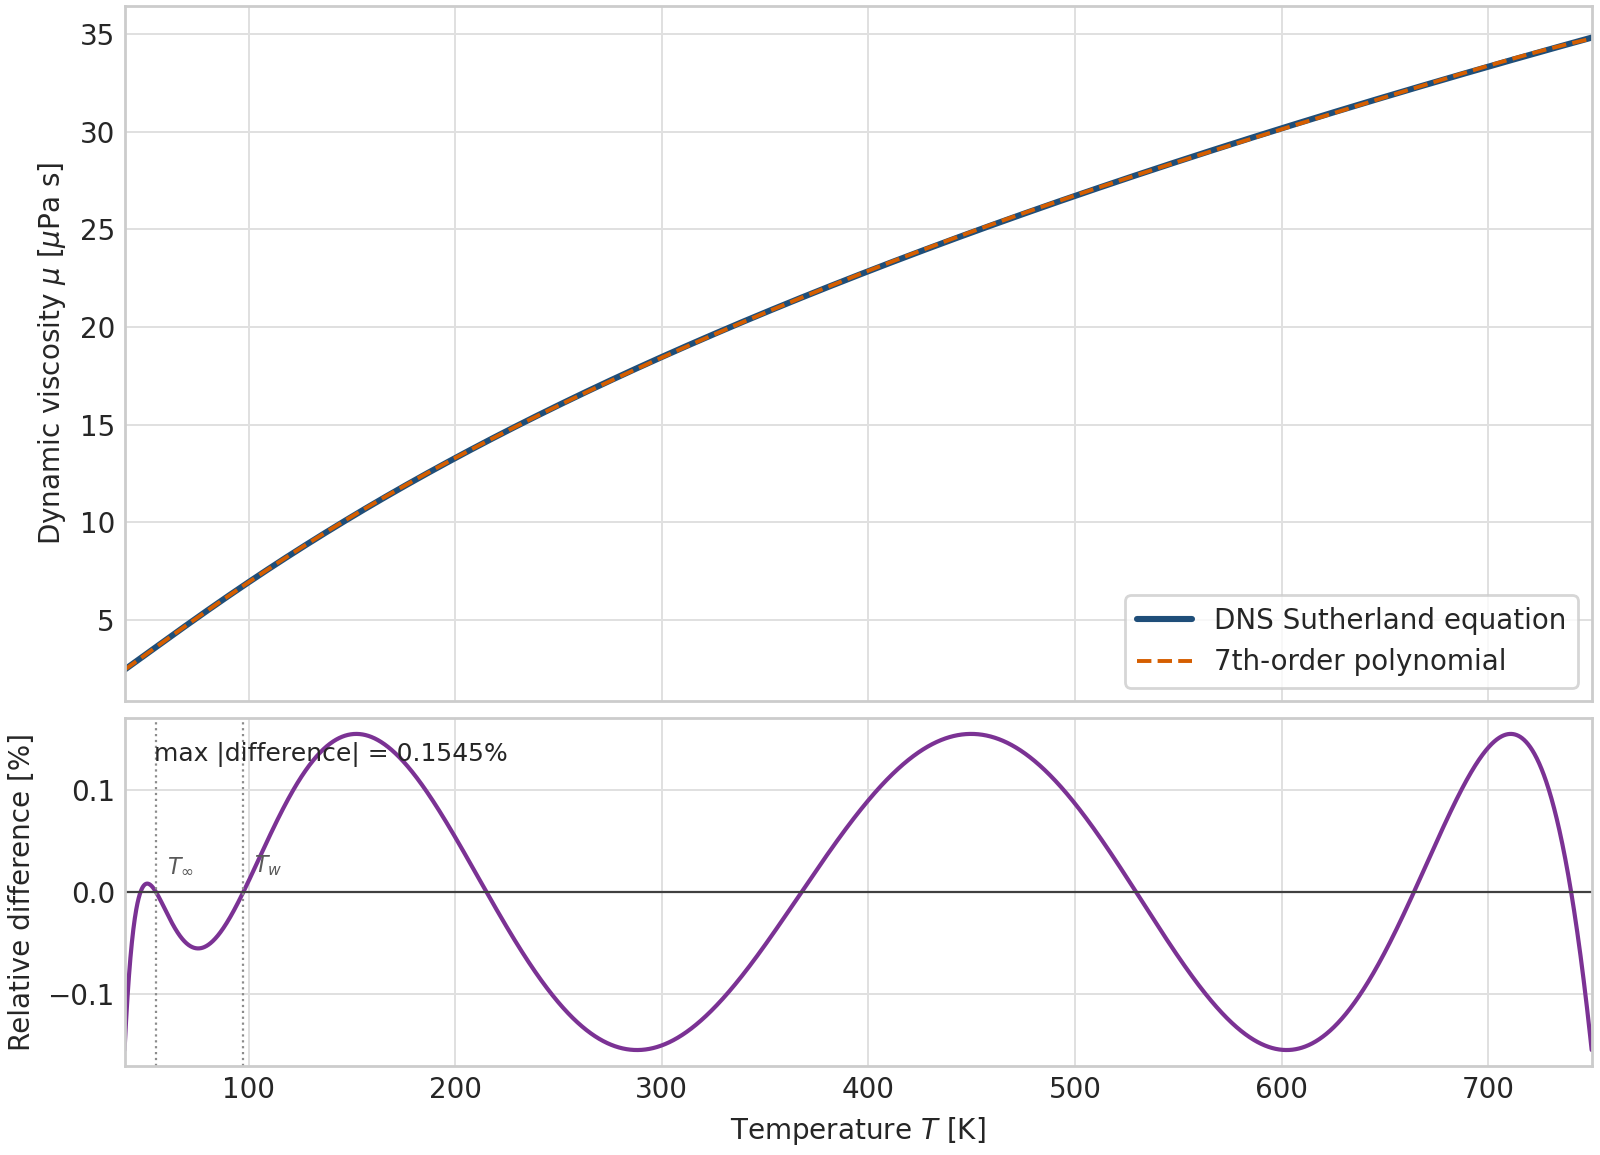
\includegraphics[width=0.8\linewidth]{06_Eval_Methodology/06_Figures/M6Tw025_sutherland_polynomial_fit.png}
    \caption{Assessment of the custom 7th-order polynomial fit for the dynamic viscosity on the M6Tw025 case, against the DNS reference's defined viscosity law. With fixed points at the \(T_w\) and \(T_\infty\).}
    \label{fig:evaluation:viscosity-fit}
\end{figure}

\paragraph*{Turbulent Prandtl number}
\label{para:turbulent-Prandtl-number}

Unless explicitly stated otherwise, the SA and \(k\)--\(\omega\) SST simulations use a constant turbulent Prandtl number \(Pr_t=0.9\). This follows common RANS practice beyond OpenFOAM: the NATO AVT-352 cone--flare comparison reports constant values of \(0.9\) for DLR TAU and NASA VULCAN, \(0.89\) for STAR-CCM+, and \(0.85\) for the Aselsan Ansys Fluent calculations~\cite[Section~IV]{hoste2025review}. NASA's LAURA manual likewise specifies \(Pr_t=0.9\) as the default~\cite[Section~5.4.17]{Thompson2024LAURA}. The present choice therefore provides a conventional baseline, retained across the benchmark set to compare the models under a common thermal-closure assumption and it is not fitted separately to each DNS case. DNS turbulent-Prandtl-number distributions and a sensitivity calculation with other constant values are discussed with the wall-resolved profile results in Section~\ref{subsec:comparative:zpg:wr-prandtl}.

\subsection{Matching station, quantities and figures of interest}
\label{subsec:evaluation:matching-station}
% Writing prerequisite for Chapter 7: keep the source-specific Re_delta2
% definitions, DNS-to-WR matching and common physical station for WF-to-WR
% comparisons explicit. Distinguish these from the Re_tau-based Pr_t sensitivity
% comparison, and distinguish q_w/tau_w from coefficients with different edge
% or freestream normalizations.


\paragraph*{On the definition of the matching station between RANS result and DNS reference}

The 12 DNS references only provide information about the boundary layer profile and the wall heat-flux and shear stress at a singular downstream station - the Huang case being the exception with providing three downstream stations. Still some studies using the same ZPG FPs, e.g. \cite{huang2019assessment}, \cite{xue2024assessment}, or \cite{aiken2022assessment} plot multiple downstream stations, although it is not traceable from these publications where exactly they got these values from. For the later sections, it is thus abstained form including them, and it is strictly adhered to comparing to the primary source's values. Still plotting the downstream development of the quantities is crucial to judging their development rather than just one snapshot. This is will become apparent on some later figures like Figure~\ref{fig:evaluation:SA-mesh-convergence-behaviour}.
\par\medskip

Another crucial point to assess, is at what spatial location to compare the RANS results with the DNS reference. This matching point can be determined by e.g. matching a physical downstream x-station, Reynolds number based on shear velocity \(Re_\tau\), Reynolds number based on momentum thickness and wall viscosity \(Re_{\delta2}\), or Reynolds number based on momentum thickness and freestream viscosity \(Re_\theta\).
\par\medskip

Matching on a physical downstream x-station is not possible because the DNS references do not provide this information with regards to the actual beginning of the boundary layer development. As the ZPG DNS cases investigated in here represent fully turbulent boundary layers and no natural or forced tripping, they are set up with predetermined turbulent boundary layers at the inlet. They subsequently report the boundary layer thickness assigned at the inlet as \(\delta_i\), and either the physical downstream sample station in the DNS domain, \(x_a\), or the ratio \(\frac{x_a}{\delta_i}\).Neither \(x_a\) or it's non-dimensionless ratio with \(delta_i\) sufficiently defines the physical downstream station in a RANS domain where the boundary layer is being developed from the leading edge onwards. Also the inlet profiles used for the DNS' are not available to exactly reproduce the domain from the same starting point.
\par\medskip

Just five weeks before hand-in of this work, Cheng et al in \cite{cheng2026reynolds} investigated the same Zhang and Huang ZPG flat-plates on RANS energy closure (see previous paragraph~\ref{para:turbulent-Prandtl-number}). Cheng et al used a novel matching station approach for their work, where they first determined the physical streamwise station at which the RANS solution produces the same boundary layer thickness as reported inflow boundary layer thickness \(\delta_i\) in the DNS references. Subsequently the DNS matched sample station is then determined by the DNS reported ratio \(\frac{x_a}{\delta_i}\), where \(x_a\) the physical downstream location in the DNS domain, from this matched boundary layer thickness \(\delta_i\). Tables~\ref{tab:evaluation:matching-station-bq} and ~\ref{tab:evaluation:matching-station-ch} however shows that the \(Re_{\delta2}\) matching chosen for this work, and a physical boundary layer distance shifted matching like done by Cheng et al., agree within 1\% for \(-B_q\) and less than 2\% for \(C_h\). 

\begin{table}[H]
    \centering
    \caption{Comparison of the dimensionless wall heat-transfer rate \(-B_q\) from DNS (D), RANS at the shifted physical matching station as proposed by Cheng et al. (S), and RANS at the \(Re_{\delta2}\)-matched station (R). Relative differences are given in percent.  The RANS solutions are from the wall-resolved \(k\)--\(\omega\) SST simulations as introduced later in Section~\ref{subsec:comparative:zpg:wr-wall-fluxes}.}
    \label{tab:evaluation:matching-station-bq}
    \small
    \setlength{\tabcolsep}{4pt}
    \begin{tabular}{@{}l S[table-format=1.2] S[table-format=1.9] S[table-format=1.9] S[table-format=-2.2] S[table-format=-2.2] S[table-format=+1.2]@{}}
        \toprule
        Case & {\shortstack{DNS (D)\\\(-B_q\)}} & {\shortstack{Shifted (S)\\\(-B_q\)}} & {\shortstack{\(Re_{\delta2}\) (R)\\\(-B_q\)}} & {\shortstack{S vs D\\{[\%]}}} & {\shortstack{R vs D\\{[\%]}}} & {\shortstack{S vs R\\{[\%]}}} \\
        \midrule
        M6Tw025  & 0.14 & 0.138455697 & 0.137434751 & -1.10  & -1.83  & +0.74 \\
        M6Tw076  & 0.02 & 0.017508213 & 0.017582069 & -12.46 & -12.09 & -0.42 \\
        M8Tw048  & 0.06 & 0.058947522 & 0.058587750 & -1.75  & -2.35  & +0.61 \\
        M14Tw018 & 0.19 & 0.186542796 & 0.185085083 & -1.82  & -2.59  & +0.79 \\
        \bottomrule
    \end{tabular}
\end{table}

\begin{table}[H]
    \centering
    \caption{Comparison of the Stanton number \(C_h\) from DNS (D), RANS at the shifted physical matching station as proposed by Cheng et al. (S), and RANS at the \(Re_{\delta2}\)-matched station (R). Relative differences are given in percent. The RANS solutions are from the wall-resolved \(k\)--\(\omega\) SST simulations as introduced later in Section~\ref{subsec:comparative:zpg:wr-wall-fluxes}.}
    \label{tab:evaluation:matching-station-ch}
    \small
    \setlength{\tabcolsep}{4pt}
    \begin{tabular}{@{}l S[table-format=1.9] S[table-format=1.9] S[table-format=1.9] S[table-format=+2.2] S[table-format=+2.2] S[table-format=+1.2]@{}}
        \toprule
        Case & {\shortstack{DNS (D)\\\(C_h\)}} & {\shortstack{Shifted (S)\\\(C_h\)}} & {\shortstack{\(Re_{\delta2}\) (R)\\\(C_h\)}} & {\shortstack{S vs D\\{[\%]}}} & {\shortstack{R vs D\\{[\%]}}} & {\shortstack{S vs R\\{[\%]}}} \\
        \midrule
        M6Tw025  & 0.001021456 & 0.001067416 & 0.001050667 & +4.50  & +2.86  & +1.59 \\
        M6Tw076  & 0.000633588 & 0.000546307 & 0.000551478 & -13.78 & -12.96 & -0.94 \\
        M8Tw048  & 0.000448561 & 0.000462389 & 0.000456311 & +3.08  & +1.73  & +1.33 \\
        M14Tw018 & 0.000243366 & 0.000282753 & 0.000277646 & +16.18 & +14.09 & +1.84 \\
        \bottomrule
    \end{tabular}
\end{table}

\begin{equation}
    Re_\tau = \frac{\rho_w u_\tau \delta}{\mu_w}
\end{equation}
Matching on the \(Re_\tau\) is seen rather often, e.g. \cite{xue2024assessment}, or \cite{aiken2022assessment}. It has the advantage that by definition of \(Re_\tau\) being calculated with the boundary layer thickness \(\delta\), this matching ensure equally thick developed boundary layer. The drawback however is that \(Re_\tau\), also relies on the shear velocity \(u_\tau\), thus any matching with \(Re_\tau\) is also an indirect matching on the skin-friction, which undermines subsequent findings on the wall shear stress behaviour. A potential ambiguity in the definition of \(Re_\tau\), is the definition of the boundary layer thickness. Whereas most often the boundary layer thickness is defined as the wall-normal distance where \(U = 99\% U_\infty\), often noted as \(\delta_{99}\), as discussed in Griffin Section~\ref{subsec:wall-functions:griffin:edge-detection}, this doesn't necessary always have to be the case, or e.g. in Huang's reference where it is rather defined as "99.5\% of the freestream total enthalpy" \cite[Nomenclature]{huang2020simulation}.

\begin{equation}
    Re_\theta = \frac{\rho_\infty u_\infty \theta}{\mu_\infty}, \qquad \text{or} \qquad Re_{\delta2} = \frac{\rho_\infty u_\infty \theta}{\mu_w},
\end{equation}
with
\begin{equation}
    \theta = \int_0^\delta \frac{\rho u}{\rho_e u_e}\left(1 - \frac{u}{u_e}\right)\,\mathrm{d}y
\end{equation}
Matching on \(Re_{\delta2}\) or \(Re_\theta\) only differs in the wether one uses the wall or freestream viscosity. The big ambiguity herein lies that sometimes the subscript-\(\infty\) freestream quantities is defined as the edge quantities, such as in the Martin-Duan cases \cite[Section 2.1]{duan2010direct_part2}. While for an ideal ZPG FP boundary layer edge and freestream should be identical, it might not be the case for more complex flows, or even for CFD where a leading edge shock imposes an ever so slight wall normal pressure gradient. The advantage is, that this matching of the momentum thickness \(\theta\), does not explicitly contain shear stress of heat-flux like \(Re_\tau\) does. Martin and Duan explicitly control for the \(Re_{\delta2}\) \cite{duan2010direct_part2}. Fernholz \& Finley explicitly favour \(Re_{\delta2}\) over the conventional \(Re_\theta\) for comparing compressible boundary layers \cite{fernholz1980critical}. Although they describe it soley as a physically motivated, empirical choice and base the momentum thickness Reynolds number on the boundary layer edge quantities.
\par\medskip

The limitation of both \(Re_\tau\) and \(Re_{\delta2}\) or \(Re_\theta\), is that neither boundary layer quantities, nor integrals across the boundary layer can be reliably determined on a coarse wall-function grid. Thus it was decided to use the \(C_f\)-independent \(Re_{\delta2}\) for matching the wall-resolved RANS turbulence model results to the DNS reference, and subsequently match the physical downstream station between wall-function and wall-resolved RANS, as ideally they both should develop the boundary layer identically. Furthermore the \(Re_{\delta2}\) equation was case-by-case carefully matched to the respective DNS paper's definition.

\paragraph*{Quantitative DNS reference data}

Table~\ref{tab:evaluation:dns-reference-values} collects the matching Reynolds number \(Re_{\delta2}\), skin-friction coefficient \(C_f\), Stanton number \(C_h\), and dimensionless wall heat-transfer rate \(-B_q\). The directly reported quantities retain the definitions, signs, and precision used in each source. Zhang's \(C_f\) values are reconstructed as described in the table notes. No conversion between \(C_h\) and \(-B_q\) is applied. Huang's three sampling stations are listed separately for the single M11Tw020 case. The corresponding CFD results and the DNS coefficient reconstructions used for their signed errors are given in Table~\ref{tab:wall-resolved:coefficients}; differences between those numerical reference values and this published-data overview are stated there.

\begin{table}[H]
    \centering
    \caption{Published and reconstructed DNS reference values for the 12 selected benchmark cases. Source keys identify the paper and the location of each quantity below the table.}
    \label{tab:evaluation:dns-reference-values}
    \small
    \begin{tabular}{@{}ll S[table-format=4.1] S[table-format=1.3,table-space-text-post={\textsuperscript{\(\dagger\)}},table-align-text-after=false] S[table-format=1.3] S[table-format=1.3]@{}}
        \toprule
        Source & Case / station & {\(Re_{\delta2}\)} & {\(10^3 C_f\)} & {\(10^3 C_h\)} & {\(-B_q\)} \\
        \midrule
        D2 & M5T1 & 1538.4 & 2.46 & 1.39 & \\
        D2 & M5T2 & 1521.5 & 2.05 & 1.14 & \\
        D2 & M5T3 & 1524.7 & 1.81 & 0.977 & \\
        D2 & M5T4 & 1526.4 & 1.50 & 0.839 & \\
        D2 & M5T5 & 1536.8 & 1.28 &  & \\
        \addlinespace
        D4 & LowH\_M3 & 1554.5 & 3.12 & 1.82 & \\
        \addlinespace
        Z & M2p5 & 1657 & 2.31{\textsuperscript{\(\dagger\)}} & & 0 \\
        Z & M6Tw025 & 1135 & 1.70{\textsuperscript{\(\dagger\)}} & & 0.14 \\
        Z & M6Tw076 & 1746 & 0.998{\textsuperscript{\(\dagger\)}} & & 0.02 \\
        Z & M8Tw048 & 1990 & 0.766{\textsuperscript{\(\dagger\)}} & & 0.06 \\
        Z & M14Tw018 & 2354 & 0.404{\textsuperscript{\(\dagger\)}} & & 0.19 \\
        \addlinespace
        H & M11Tw020 (BL1) & 2204 & 0.61 & 0.36 & 0.164 \\
        H & M11Tw020 (BL2) & 3419 & 0.55 & 0.32 & 0.154 \\
        H & M11Tw020 (BL3) & 4390 & 0.51 & 0.29 & 0.148 \\
        \bottomrule
    \end{tabular}
    \par\smallskip
    \begin{minipage}{\linewidth}
        \footnotesize
        \textbf{D2:} Martin-Duan Part 2~\cite{duan2010direct_part2}: \(Re_{\delta2}\) in Table~1 (p.~421); \(C_f\) and \(C_h\) in Table~3 (p.~425).
        \par
        \textbf{D4:} Martin-Duan Part 4~\cite{duan2011direct_Part4}: \(Re_{\delta2}\) in Table~2 (p.~31); \(C_f\) and \(C_h\) in Table~4 (p.~42).
        \par
        \textbf{Z:} Zhang et al.~\cite{zhang2018direct}: \(Re_{\delta2}\), \(-B_q\), and \(u_\tau\) from Table~2; \(U_\infty\) from Table~1 (p.~4299). Entries marked \(\dagger\) use \(C_f=2(\rho_w/\rho_\infty)(u_\tau/U_\infty)^2\), with \(\rho_\infty/\rho_w\) from the outermost digital DNS profile point. Coefficients are rounded to three significant figures.
        \par
        \textbf{H:} Huang et al.~\cite{huang2020simulation}: \(Re_{\delta2}\) and \(-B_q\) from Table~3; \(C_f\) and \(C_h\) from Table~4 (both p.~11).
    \end{minipage}
\end{table}

Zhang et al. report \(-B_q\) to only two decimal places in both the paper~\cite[Table~2, p.~4299]{zhang2018direct} and the accompanying digital data headers. Assuming rounding to the nearest \(0.01\), this reporting precision implies an absolute rounding bound of \(\pm0.005\). Table~\ref{tab:evaluation:zhang-bq-rounding} gives the corresponding intervals and relative bounds for the four nonzero values. The effect is particularly pronounced for M6Tw076: its reported value of \(-B_q=0.02\) has a rounding bound of \(\pm25\%\) relative to that value. Since the reconstructed wall heat-flux and Stanton number are proportional to \(B_q\) when the other inputs are held fixed, the same relative bound applies to these quantities. This reporting precision therefore limits quantitative heat-flux validation based on the tabulated \(-B_q\) values, particularly for M6Tw076, but also a \(\pm3.57\%\) is significant, when the goal is to achieve a \(\pm5\%\) heat-flux prediction accuracy \ref{sec:evaluation:success-criteria}. Thus and because of the aforementioned ambiguity and mismatch in the reported wall temperature, the M6Tw076 is being excluded from heat-flux assessments.

\begin{table}[H]
    \centering
    \caption{Rounding bounds for Zhang et al.'s reported \(-B_q\) values, assuming rounding to the nearest \(0.01\).}
    \label{tab:evaluation:zhang-bq-rounding}
    \small
    \begin{tabular}{@{}l S[table-format=1.2] S[table-format=1.3,table-number-alignment=right]@{\,--\,}S[table-format=1.3,table-number-alignment=left] S[table-format={\pm2.2},table-space-text-post={\%},table-align-text-after=false]@{}}
        \toprule
        Case & {Reported \(-B_q\)} & \multicolumn{2}{c}{Rounding interval} & {Relative bound} \\
        \midrule
        M6Tw025 & 0.14 & 0.135 & 0.145 & \pm3.57{\%} \\
        M6Tw076 & 0.02 & 0.015 & 0.025 & \pm25.0{\%} \\
        M8Tw048 & 0.06 & 0.055 & 0.065 & \pm8.33{\%} \\
        M14Tw018 & 0.19 & 0.185 & 0.195 & \pm2.63{\%} \\
        \bottomrule
    \end{tabular}
    \par\smallskip
    \begin{minipage}{\linewidth}
        \footnotesize
        Relative bounds are calculated as \(0.005/|B_{q,\mathrm{reported}}|\) and expressed as percentages of the reported value.
    \end{minipage}
\end{table}

\paragraph*{Qualitative DNS reference figures}

The reference figures of interest for this work are particularly the boundary layer profiles. For the Zhang cases these are taken directly from the downloadable digital data, thus providing a high quality reference, with no digitization errors, and very fine resolution.
\par\medskip

The M11Tw0120 reference case by Huang et al has been published with the momentum and thermal boundary layer profile in \cite[Figure 12(a), Figure 13(a)]{huang2020simulation}, but only for the BL2, downstream station.
\par\medskip

For Martin--Duan Part~2, the van Driest--transformed velocity profiles and \(T(U)\) relations are digitized from Figures~5 and 6, respectively~\cite{duan2010direct_part2}. The wall levels in Figure~6, interpreted alongside Table~1, suggest mixed temperature normalization: \(T/T_\delta\) for M5T1, with \(T_\delta=228.1\,\mathrm{K}\), and \(T/T_\infty\) for M5T2--M5T5, with nominal \(T_\infty=216.65\,\mathrm{K}\)~\cite[Table~1]{martin2007direct_Part1}. Velocity remains normalized as \(U/U_\delta\) for all five cases and is dimensionalized using each case's tabulated edge state. This mixed interpretation is inferred here from the wall levels and tabulated conditions. Contacting the authors to confirm this accidentally mixed normalization yielded no response, from the clear requirement of the thermal boundary layer profiles to match the prescribed wall temperature at the wall, this inferred correction is reasonable. For Part~4 LowH\_M3, Figure~7 supplies the transformed velocity profile, while Figure~8 is dimensionalized using the tabulated edge temperature and velocity~\cite{duan2011direct_Part4}.
\par\medskip

For future reusing of these DNS reference cases it should also be noted, that Zhang and Huang define the dimensionless wall shear stress coefficient \(C_h\) and the Stanton number \(C_h\) via the freestream quantities \cite[Nomenclature]{zhang2018direct,huang2020simulation}, whereas Martin and Duan use the boundary layer edge quantities \cite[p.424]{duan2010direct_part2}, for their cases the quantities at 99\% freestream velocity \cite[p. 421]{duan2010direct_part2}
\par\medskip

The separate inconsistency between the Martin-Duan Part~2 Reynolds-number columns and the resulting limitation of \(Re_{\delta2}\) as a nominal matching target are discussed in Appendix~\ref{app:duan:reynolds}.

\section{Wall-resolved mesh requirements}
\label{sec:evaluation:mesh-families-yplus}

Wall-resolved RANS meshes are commonly designed to place the first cell centre at \(y_1^+\le1\). The NASA Turbulence Modeling Resource describes this as conventional practice for simulations that integrate the turbulence model to the wall.\footnote{\url{https://tmbwg.github.io/turbmodels/flatplate_val_ypluseffect.html}} A general basis for treating this rule as sufficient for hypersonic cold-wall heat-flux convergence was not identified in the literature reviewed here. Fletcher~\cite[p.~401]{fletcher2012computational}, for example, recommends \(y^+<5\) to resolve the near-wall velocity profile and notes that compressible temperature profiles may require \(y^+<2\). These recommendations motivate placing the first point within the viscous sublayer, but do not establish a convergence criterion for heat-transfer under hypersonic cold-wall conditions.
\par\medskip

The first-cell centre lies at \(y_1=\delta_n=\Delta y_1/2\) for the
wall-normal cells used here, where \(\Delta y_1\) is the full first-cell
thickness. Its distance in wall units is \(y_1^+=\rho_w u_\tau y_1/\mu_w\),
with friction velocity \(u_\tau=\sqrt{|\tau_w|/\rho_w}\).
The alternative resolution indicator is the first-cell acoustic Reynolds number
\begin{equation}
    Re_{\mathrm{cell1}}=\frac{\rho_w a_w\,\delta_n}{\mu_w}.
    \label{eq:evaluation:first-cell-acoustic-re}
\end{equation}
Here \(\rho_w\), \(a_w\) and \(\mu_w\) are the density, speed of sound and
dynamic viscosity evaluated at the wall.

Dilley~\cite{dilley2001evaluation} found that a cell Reynolds number of approximately unity was required for grid-converged hypersonic heating predictions with the Baldwin--Lomax model. His definition uses first-cell properties and the full cell height, so its numerical threshold cannot be transferred directly to Equation~\eqref{eq:evaluation:first-cell-acoustic-re}, but it gives an indication. Related criteria have also been used for laminar stagnation-point heating~\cite{papadopoulos1999current}, aeroheating calculations for the X-38~\cite{loomis2004aeroheating} and mesh adaptation in LAURA~\cite{Thompson2024LAURA}.
\par\medskip

Figures~\ref{fig:evaluation:SA-mesh-convergence-behaviour} and~\ref{fig:evaluation:SST-mesh-convergence-behaviour} illustrate the effect of reducing the first-cell height for M6Tw025. They show the streamwise development of the skin-friction coefficient \(C_f\) and Stanton number \(C_h\), expressed in terms of \(Re_\tau\), at fixed downstream spacing. For SA, the curves nearly coincide from \(y_1^+=1.24\) down to the finest mesh. The \(k\)--\(\omega\) SST model requires refinement to approximately \(y_1^+=0.129\) before mesh convergence is reached. The weaker first-cell sensitivity of SA is qualitatively consistent with the NASA flat-plate study cited above, which reports greater sensitivity for models using an \(\omega\) equation.

\begin{figure}[H]
    \centering
    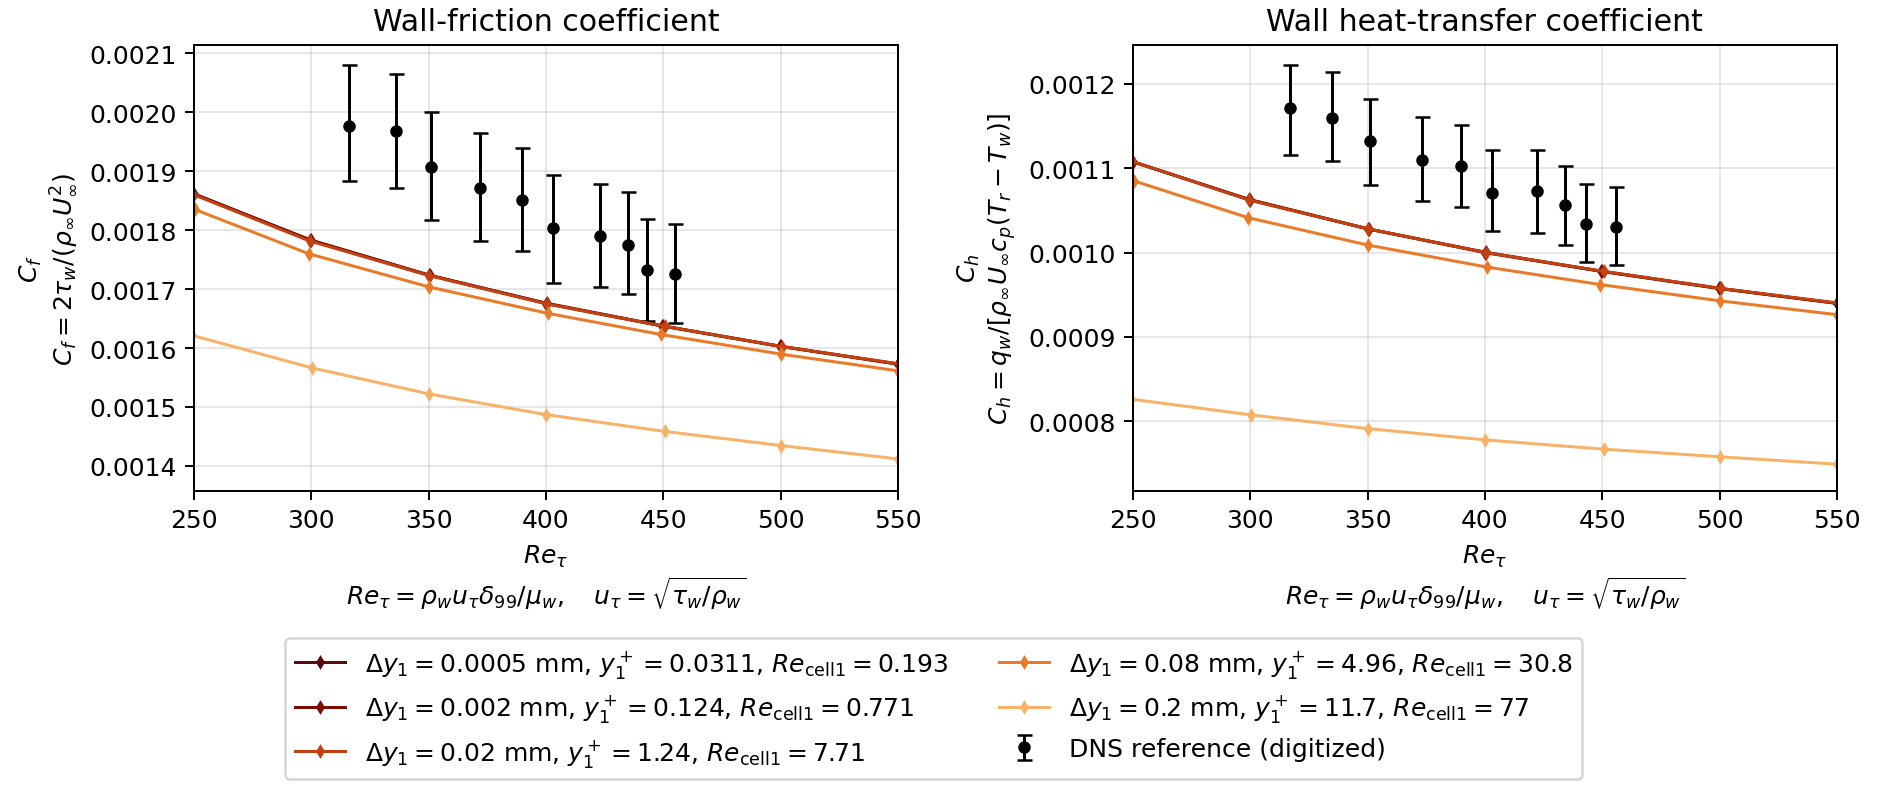
\includegraphics[width=\linewidth]{06_Eval_Methodology/06_Figures/SA_wall_coefficients_vs_dns.png}
    \caption[M6Tw025: first-cell mesh sensitivity with SA]{First-cell mesh sensitivity of the SA predictions for M6Tw025: skin-friction coefficient \(C_f\) (left) and Stanton number \(C_h\) (right) versus \(Re_\tau\), with fixed downstream spacing \(\Delta x=5\,\mathrm{mm}\). Coloured curves show the different first-cell thicknesses \(\Delta y_1\); black symbols denote the digitized DNS reference~\cite{zhang2018direct}. The \(y_1^+\) values reported in the legend are evaluated at each mesh's DNS-matched station, defined by \(Re_{\delta2}=1135\), rather than representing a constant value along the plate.}
    \label{fig:evaluation:SA-mesh-convergence-behaviour}
\end{figure}

\begin{figure}[H]
    \centering
    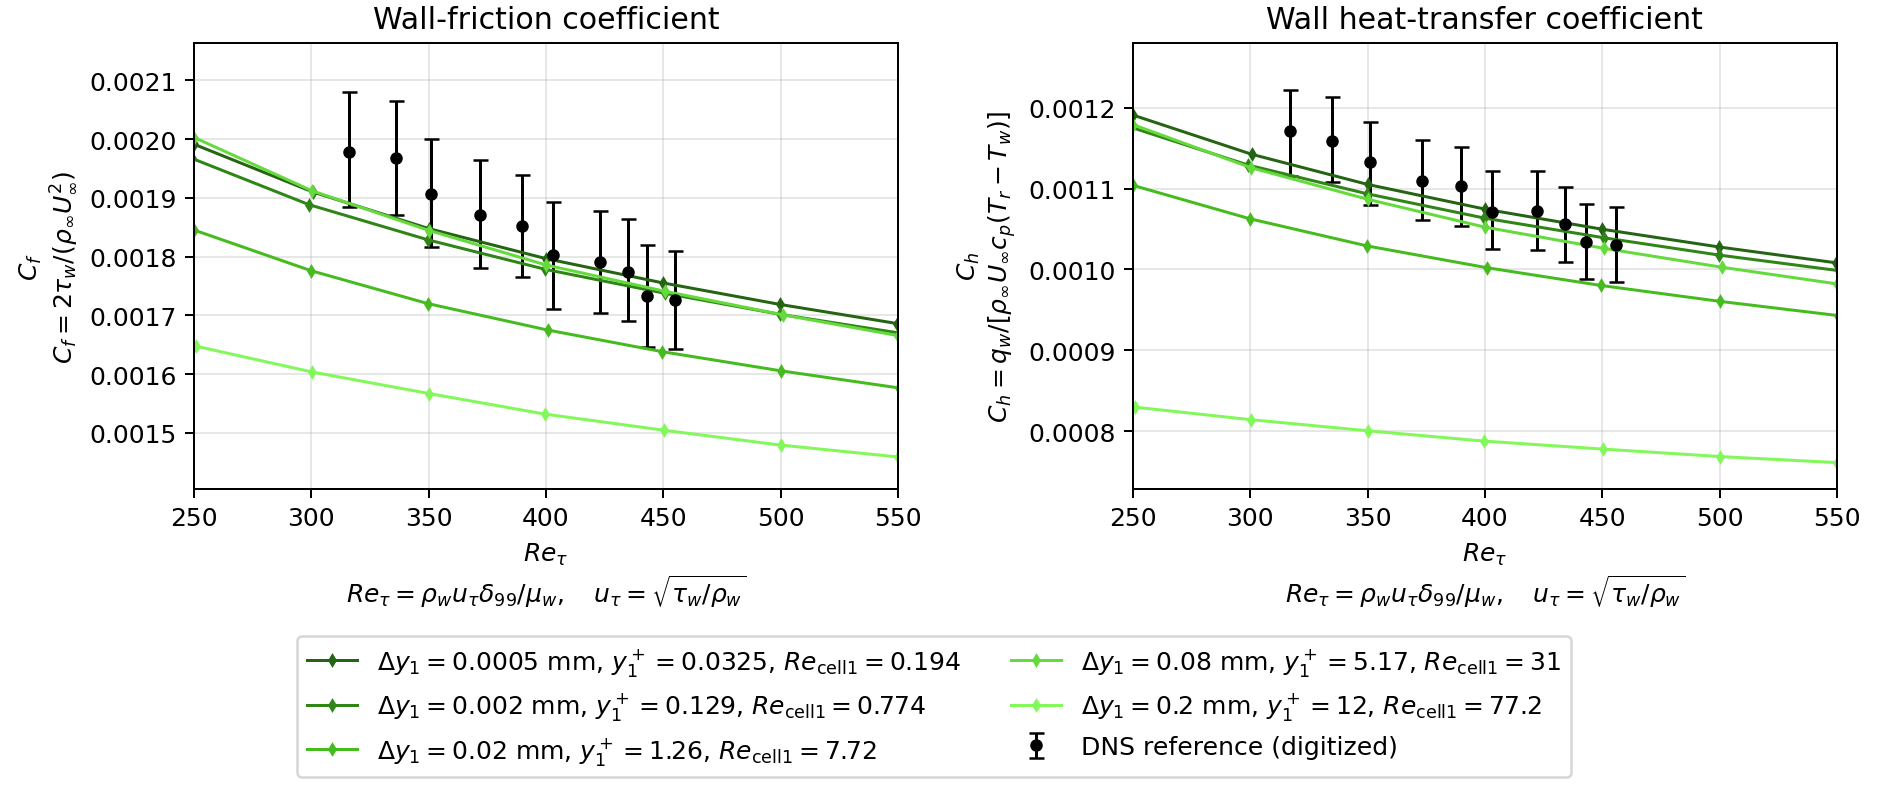
\includegraphics[width=\linewidth]{06_Eval_Methodology/06_Figures/kwSST_wall_coefficients_vs_dns.png}
    \caption[M6Tw025: first-cell mesh sensitivity with SST]{First-cell mesh sensitivity of the \(k\)--\(\omega\) SST predictions for M6Tw025: skin-friction coefficient \(C_f\) (left) and Stanton number \(C_h\) (right) versus \(Re_\tau\), with fixed downstream spacing \(\Delta x=5\,\mathrm{mm}\). Coloured curves show the different first-cell thicknesses \(\Delta y_1\); black symbols denote the digitized DNS reference~\cite{zhang2018direct}. The \(y_1^+\) values reported in the legend are evaluated at each mesh's DNS-matched station, defined by \(Re_{\delta2}=1135\), rather than representing a constant value along the plate.}
    \label{fig:evaluation:SST-mesh-convergence-behaviour}
\end{figure}

Appendix~\ref{app:zpg:mesh-convergence} extends the wall-normal refinement study to all twelve ZPG flat-plate cases. Streamwise-refinement tests for M6Tw025 showed negligible sensitivity of heat-flux and skin-friction to the downstream spacing when the leading edge was refined. The remaining mesh studies therefore focus on the wall-normal direction. They report skin-friction and, for the isothermal cases, heat-transfer against \(y_1^+\) and \(Re_{\mathrm{cell1}}\) at the DNS-matched downstream stations. For the investigated hypersonic cold-wall cases, these results support \(Re_{\mathrm{cell1}}\le1\) as a practical resolution guideline, particularly for SST, in preference to relying on \(y_1^+\le1\) alone.
\par\medskip

The wall-gradient approximation provides a plausible explanation for this stringent resolution requirement. As discussed in Section~\ref{sec:openFOAM_qw_tauw}, OpenFOAM/HiSA evaluates the wall gradients from the difference between the wall value and the first off-wall cell value. Accurate wall fluxes therefore require this secant to approximate the local wall derivative. Placing the first cell within the nominal viscous sublayer is insufficient if the velocity or temperature gradient varies appreciably across that distance. The cold-wall profile shapes in Figures~\ref{fig:background:dns-velocity-profiles} and~\ref{fig:background:dns-temperature-profiles} motivate this distinction between resolving a profile and resolving its wall slope. The mesh studies establish the numerical basis for the wall-resolved model comparisons in Section~\ref{sec:comparative:zpg:wall-resolved-baselines}, where agreement with the DNS reference is assessed separately there.

\section{Criteria for successful performance}
\label{sec:evaluation:success-criteria}
% Writing prerequisite for Chapter 7: finalize the accuracy targets and their
% rationale, including the plotted +/-5% DNS-relative target band. Distinguish
% an engineering acceptance target from DNS uncertainty or reporting precision.

Section~\ref{sec:evaluation:benchmark-cases} identifies uncertainties and ambiguities in the DNS references used for this assessment. In comparing RANS predictions with these references, as in related assessments such as that of Xue et al.~\cite{xue2024assessment}, a quantitative accuracy target is needed. This work adopts a \(\pm5\%\) DNS-relative error band as the target for wall-resolved heat-flux predictions. This band is an engineering acceptance criterion and neither represents the uncertainty of the individual DNS references nor defines a statistical confidence interval. The reference limitations discussed above must therefore be considered when judging agreement within this band.
\par\medskip

The target is motivated by the relative simplicity of attached ZPG flat-plate boundary layers and the accuracy already achieved by analytical approaches. Hasan et al.~\cite[Figure~2]{manzoor2024estimating}, for example, report heat-transfer errors mostly within \(\pm8\%\), with a maximum of \(10.3\%\), for a dataset that includes several of the benchmarks investigated here. Wall-resolved RANS should therefore aim to improve on this level of accuracy. For wall-function calculations, \(\pm10\%\) is adopted as the minimum acceptable heat-flux accuracy: for these ZPG cases, larger errors would leave the additional computational cost of CFD without a corresponding gain in heat-flux accuracy over the analytical approach.
\par\medskip

Beyond error magnitude, engineering use also requires an assessment of how consistently a method behaves. A systematic bias is easier to account for than an error that varies strongly and non-monotonically with sampling height or mesh spacing. This distinction helps frame the three analyses that follow: wall-resolved RANS discrepancies in Section~\ref{sec:comparative:zpg:wall-resolved-baselines}, wall-function closure errors in Section~\ref{sec:comparative:zpg:cross-comparison}, and spatial-discretization errors in Section~\ref{subsec:comparative:zpg:yplus-sensitivity}. For example, the wall-resolved heat-flux discrepancy for a given case may act primarily as a bias, while the closure and spatial discretization may introduce more irregular variations as the sampling height and mesh spacing change. The following sections examine these behaviours alongside the quantitative accuracy targets.

